%%%%%%%%%%%%%%%%%%%%%%%%%%%%%%%%%%%%%%%%%%%%%%%%%%%%%%%%%%%%%%%%%%%%%%%%%%%%%%%%
%2345678901234567890123456789012345678901234567890123456789012345678901234567890
%        1         2         3         4         5         6         7         8

\documentclass[a4, 10 pt, conference]{ieeeconf}  % Comment this line out if you need a4paper

%\documentclass[a4paper, 10pt, conference]{ieeeconf}      % Use this line for a4 paper

\IEEEoverridecommandlockouts                              % This command is only needed if 
                                                          % you want to use the \thanks command

\overrideIEEEmargins                                      % Needed to meet printer requirements.

% See the \addtolength command later in the file to balance the column lengths
% on the last page of the document

% The following packages can be found on http:\\www.ctan.org
%\usepackage{graphics} % for pdf, bitmapped graphics files
%\usepackage{epsfig} % for postscript graphics files
%\usepackage{mathptmx} % assumes new font selection scheme installed
%\usepackage{times} % assumes new font selection scheme installed
%\usepackage{amsmath} % assumes amsmath package installed
%\usepackage{amssymb}  % assumes amsmath package installed
\usepackage{multicol}
\usepackage{tcolorbox}
\usepackage{cuted,tcolorbox,lipsum}
\usepackage{xcolor}
\usepackage{hyperref}
\usepackage{graphicx}

\title{\LARGE \bf
Introduction to Machine Learning (SS 2025)\\ Programming Project
\vspace{-3em}
}


\begin{document}


\maketitle
\vspace{-3em}
\thispagestyle{empty}
\pagestyle{empty}

\begin{strip}
\begin{tcolorbox}[
size=tight,
colback=white,
boxrule=0.2mm,
left=3mm,right=3mm, top=3mm, bottom=1mm
]
{\begin{multicols}{2}% replace 3 with 2 for 2 authors.

\textbf{Author 1}\\
Last name: Gajdos\\
First name: Dominik\\
Matrikel Nr.: 12311949\\  

\columnbreak

\textbf{Author 2}\\
Last name: Wintner\\
First name: Patrick\\
Matrikel Nr.: 12143491\\

\end{multicols}}
\end{tcolorbox}
\end{strip}

%%%%%%%%%%%%%%%%%%%%%%%%%%%%%%%%%%%%%%%%%%%%%%%%%%%%%%%%%%%%%%%%%%%%%%%%%%%%%%%%

\section{Introduction}
\label{sec:intro}
This report is covers the detection of fraudulent transactions using different binary classifiers. The dataset has 30 features and contains more than 227,800 entries belonging either to class 0 (not fraudulent) or 1 (fraudulent). The dataset is extremely imbalanced; roughly 99.8\% of all transactions are not fraudulent. All features are numerical.

\section{Implementation / ML Process}
\label{sec:methods}
We decided to implement logistic regression and a random forest for this task. Both methods are binary classifiers and thus appropriate for this problem. Furthermore, random forests are recommended by Baeldung for fraud detection\cite{baeldung}. Each model has been implemented by one author, which has resulted in slightly different approaches for each classifier.

\subsection{Data Logistic Regression}
\subsubsection{Data-Preprocessing}
\label{subsubsection:data-processing}
First, we computed the absolute correlation of each feature with the target class (Class) and selected the top N features most correlated with the fraud label. 

\begin{table}[h!]
\begin{tabular}{l r}
\hline
\textbf{Correlation} & \textbf{Feature} \\
\hline
$>$ 0.3 		& F16, F13 \\
0.3 - 0.2  	& F11, F9, F15 \\
0.2 - 0.09 	& F2, F6, F10, F3, F17, F0, F8, F4, F1 \\
$<$ 0.05 	& Remaining Features \\
\hline
\end{tabular}
\centering
\caption{Top and Bottom Correlated Features with 'Class'}
\end{table}

Features with high a correlelation have a strong linear relationship with the target, low correlation have a weak linear relationship. Choosing features with higher correlation often leads to better performance in models while low correlation may lead to unnecessary noise. In testing, it has been shown that the top 12 features deliver the best F1 score, while the top 26 features deliver the best ROC-AUC score.
The features were then scaled using StandardScaler to normalize their distributions. No data augmentation or dimensionality reduction (e.g., PCA) was applied, as the dataset was already anonymized and numerical.

\subsubsection{Classifier Properties}
\label{subsubsection:classifier-properties}
As fraud detection in this example is a binary classification problem (1 - fraud, 0 - not fraud), Logistic Regression has been used to estimate the probability of a transaction being classified as fraudalent. The model works by calculating a weighted linear combination of the input features and then applying the logistic (sigmoid) function to transform this linear output into a probability value, in this case 0 or 1.

As the dataset is very imbalanced — where fraudulent transactions are much rarer compared to legitimate ones — the model was configured with the \texttt{class\_weight='balanced'} parameter. It adjusts the weight of each class inversely proportional to their frequency in the training data, decreasing bias towards the majority class.

\subsubsection{Hyperparameters}
\label{subsubsection:hyperparameters}
This method focuses on three hyperparameters: test size, number of features and threshold. Firstly the test size is set between 20$%$ and 40$%$, as everything above and below did not yield useful results. Secondly, as stated in the Data Processing section, the number of features has been set between 3-27 features. Lastly, as tweaking the threshold has no effect on the ROC-AUC score, the refinement of it only leads to better F1 results. 

The ROC AUC score provides a single scalar value summarizing the models ability to distinguish between the two classes 
across all possible classification thresholds. Unlike accuracy, it is not biased by class imbalance.

\begin{figure}[h!]
  \centering
  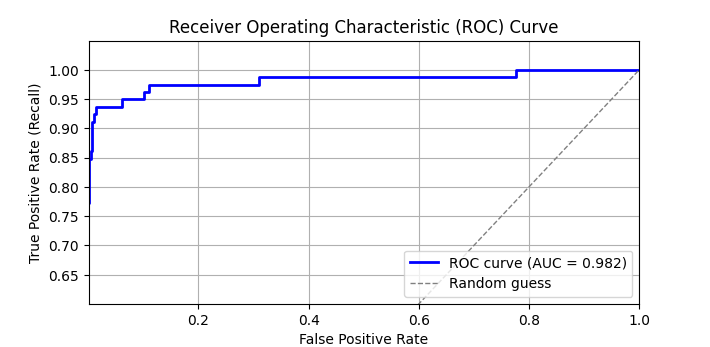
\includegraphics[width=0.5\textwidth]{roc_auc_curve.png}
  \caption{ROC curve for the logistic regression model evaluated on the best set of hyperparameters. Number of Features: 26, Test Set Size: 0.2, Train ROC-AUC: 0.985, Test ROC-AUC: 0.982}
  \label{fig:roc}
\end{figure}

\begin{table*}[hbt]
	\centering
	\begin{tabular}{c|c|c|c|c}
		& $n\_components$ & $n\_estimators$ & $max\_features$ & $criterion$\\
		\hline range & $\{1, 7, 13,\dots , 25\}$ & $\{10, 11,\dots, 100\}$ & $[0,1]$ & $\{gini, entropy, log\_loss\}$\\
		\hline choice & 19 & 47 & 0.225 & log\_loss
	\end{tabular}
	\caption{Hyperparameter selection random forest}
	\label{tab:param.rf}
\end{table*}

The curve shows the trade-off between the true positive rate and false positive rate across different thresholds. The area under the curve (AUC) is approximately 0.982, indicating strong performance in distinguishing fraudulent from legitimate transactions.



\subsection{Random Forest}
The implementations of principal component analysis and random forests of scikit-learn are used.
\subsubsection{Data-Preprocessing}
\label{subsubsection:data-processing}
The data is split into a training and test set, which contain 75\% and 25\% of all samples respectively. The dimensionality of the input data is reduced by using principal component analysis. The implementation of scikit-learn uses singular value decomposition without scaling the input data beforehand \cite{sl.pca}. The number of dimensions kept is determined via randomized search cross validation (see \ref{subsubsection:hyperparameters}); the other parameters are kept to their default values.
\subsubsection{Classifier Properties}
\label{subsubsection:classifier-properties}
Each tree in the ensemble is built from a sample drawn with replacement and using the best split strategy. The final prediction is the average of the probabilistic predictions of the individual trees (instead of using a voting mechanism). The most important hyperparameters according to the scikit-learn documentation are the number of trees in a forest and the number of features used to determine the best split \cite{sl.rf}. Those are determined via randomized search cross validation (see \ref{subsubsection:hyperparameters}), as is the criterion used to measure the impurity of a split. The other parameters are kept to their default values, therefore there is no maximal tree depth, no maximal number of leaf nodes and classes are not weighted.
\subsubsection{Hyperparameters}
\label{subsubsection:hyperparameters}
The most important hyperparameters (for search ranges and final choices see table \ref{tab:param.rf}) are determined by using the implementation of randomized search cross validation provided by scikit-learn. The randomized search cross validation is given a pipeline consisting of a PCA-Object and a random forest classifier. Five-fold cross-validation is used as cross-validation scheme and the ROC AUC score is used for performance measurement. Ten different parameter settings are sampled. The pipeline is refitted with the best parameters found.

K-fold cross validation works by splitting the training set into k smaller sets, training the model on k-1 sets and using the last set for validation. This is done k times so that each set is used once for validation. The performance is then computed by taking the average. \cite{sl.cv}

The implementation of randomized Cross validation search by scikit-learn optimizes parameters by sampling a number of parameter settings of a given parameter space, performing cross validation for the sampled setting, and keeping the parameters that resulted in the best score. Using a pipeline allows several steps (e.g. data-preprocessing followed by a classifier) to be cross-validated together. \cite{sl.rcv}

\section{Results}
\label{sec:results}
Both classifiers achieve acceptable results on the validation set, which can be seen in table \ref{tab:results}.

\begin{table}[h]
\centering
\begin{tabular}{c|c|c|c|c}
Classifier & ROC-AUC & Accuracy & Precision & Recall\\
\hline logistic regression & 98.5\% &  97.4\% & 86.8\% & 74.7\% \\
\hline random forest & 91.6\% & 99.97\% & 97.4\% & 83.1\%
\end{tabular}
\caption{Validation scores}
\label{tab:results}
\end{table}

\section{Discussion}
\label{sec:discuss}

\subsection{Logistic Regression}
\subsection{Random Forest}
The parameters determined by randomized cross-validation search lead to slightly better results than the default parameters. It however is computionally way more expensive.

The most obvious way to improve the results is to sample more parameter settings during randomized cross-validation search and by using tighter bounds for the spaces from wich the parameters are sampled. Another option to likely increase the performance is to set the parameter \emph{class\_weight} of the random forest classifier to 'balanced\_subsample' to take the imbalance of the dataset into account.

Surprisingly, the effect on performance of using principal component analysis is negligible. This is probably because the parameter max\_features, which determines the number of features used for determining the best split has a somewhat similar effect (reducing the number of relevant features). Interestingly, the chosen values for n\_components and for max\_features result in a number of relevant features, which is near default value of max\_features=$\sqrt{n\_features}$ \cite{sl.rf} without PCA: $n\_components*max\_features = 19*0.225 \approx 4.3$ and $max\_features\_default=\sqrt{n\_features}=\sqrt{30}\approx 5.5$.

\section{Conclusion}
\label{sec:con}
The final test performance with the random forest classifier is $\approx$ 0.893 and thus slightly worse than the score on the validation set. Both classifiers seem to be valid choices for fraud detection with similar performance.

It is somewhat surprising that randomized cross validation search with few trials can find parameters that results in slightly better performance than recommended default values. Considering the suggested improvements in \ref{sec:discuss}, the performance gap can likely be further increased. This suggests that randomized cross validation search is a good alternative to the computionally more expensive exhaustive grid search.

\begin{thebibliography}{xxxx}
	\bibitem{baeldung} \url{https://www.baeldung.com/cs/random-forest-vs-extremely-randomized-trees} [online; last access on 02.07.2025]
	\bibitem{sl.pca} \url{https://scikit-learn.org/stable/modules/generated/sklearn.decomposition.PCA.html} [online; last access on 02.07.2025]
	\bibitem{sl.rf} \url{https://scikit-learn.org/stable/modules/ensemble.html#random-forests-and-other-randomized-tree-ensembles} [online; last access on 02.07.2025]
	\bibitem{sl.cv} \url{https://scikit-learn.org/stable/modules/cross_validation.html#cross-validation} [online; last access on 03.07.2025]
	\bibitem{sl.rcv} \url{https://scikit-learn.org/stable/modules/grid_search.html#randomized-parameter-search}
\end{thebibliography}
%%%%%%%%%%%%%%%%%%%%%%%%%%%%%%%%%%%%%%%%%%%%%%%%%%%%%%%%%%%%%%%%%%%%%%%%%%%%%%%%

\end{document}
